% Use this file as a template for your text. Updated 18/03/2022.
% You may use your \newcommands placed in the marked space below
% Do not use separate files with macros

% Before processing this file, please make sure that the file
% aadmbook.cls is in the same folder with this file.
% The file aadmbook.cls can be downloaded from http://pefmath.etf.rs/aadmbook.cls

\documentclass[leqno]{aadmbook}
\usepackage{amsthm}
\usepackage{amsfonts}
\usepackage{amsmath}
\usepackage{graphicx}
\usepackage{amsmath, amsthm, amsfonts, amssymb}
\usepackage{float} %package for figure and table placement 
%all necessary packages should be here

\graphicspath{{paper_images/}}
\newtheorem{theorem}{Theorem}
\newtheorem{notice}{Remark}


\newcounter{definition}[section]
\newenvironment{definition}[1][]{\refstepcounter{definition}\par\medskip
    \noindent \textbf{Definition~\thedefinition. #1} \rmfamily
}
{\medskip}

\renewcommand{\mod}[1]{\textrm{mod}\ #1}

\pagestyle{myheadings}

\textwidth 28cc

\markboth{{\small\rm \hfill O.V. Arutyunov, V.A. Skorokhodov - header
\hfill}\hspace{-\textwidth}%
\underline{${{}_{}}_{}$\hspace{\textwidth}}}
{\underline{${{}_{}}_{}$\hspace{\textwidth}}\hspace{-\textwidth}%
{\small\rm \hfill Metagraph approach for construction of an (m, n)-regular bipartite graph with a given girth
\hfill}}

\setcounter{page}{1}
%\hoffset=-2.0em
\textheight 42cc

\parskip .5mm

\parindent 2cc

\begin{document}

% Your \newcommands below (if there are any):

\oddsidemargin 16.5mm
\evensidemargin 16.5mm

\thispagestyle{plain}

\begin{center}
{\large \sc  Applicable Analysis and Discrete Mathematics}

{\small available online at  http:/$\!$/pefmath.etf.rs }
\end{center}

\noindent{\small{\sc  Appl. Anal. Discrete Math.\ }{\bf x} (xxxx),xxx--xxx.}\\
\noindent{\scriptsize https://doi.org/10.2298/AADMxxxxxxxx}     %%%%%%%%%%%%%%%%%%%%%%%%%%%%%%%%%%%%%%%%%%%%

\vspace{5cc}
\begin{center}

{\large\bf  METAGRAPH APPROACH FOR CONSTRUCTION OF AN (M, N)-REGULAR BIPARTITE GRAPH WITH A GIVEN GIRTH
\rule{0mm}{6mm}\renewcommand{\thefootnote}{}%Enter at least one, but not more than 3 MSCs.
% First entered MSC will be a primary one, others (at most 2) will be secondary.


\footnotetext{\scriptsize ${}^{\ast}$Corresponding author. Oleg Arutyunov}
\footnotetext{\scriptsize 2020 Mathematics Subject Classification. 05C38, 05C90, 94B15.

\rule{2.4mm}{0mm} Keywords and Phrases. Bipartite graphs, girth, metagraphs, construction of graphs, regular graphs.}}

\vspace{1cc}
{\large\it Oleg Arutyunov, Vladimir Skorokhodov}

\vspace{1cc}
\parbox{24cc}{{\small

Short abstract here (not more than 7 lines of text)

%Avoid citations in the  abstract, but if they are necessary, do not use labels from the
%main body of the article. For example, instead of  writing "formula (2)" , you
%should reproduce formula (2), or describe it in words. Instead of writing
%"the result  obtained in [1]" , you should write "the result obtained in
%{\sc J. A. Baker:}  {\it Isometries in normed spaces,}
%Amer. Math. Monthly {\bf 78} (1971), 655--658".

}}
\end{center}

% The paper should have at least two sections

%TODO: Сделать секции как в шаблоне

% \vspace{1.5cc}
% \begin{section}
% {FILL SECTION TITLE HERE}
% \end{section}

\section{Introduction}

Many modern algorithms of data encoding use bipartite graphs with specific properties for error correction during data transmission over noise channels, e.g. Low Density Parity Check Codes \cite{johnson} \cite{ldpc_encoding}. 

% Нужна ли цитата для переборного алгоритма, а то она потерялась
Methods of construction for such bipartite graphs are divided in two main categories: methods, based on random permutations of different graphs, e.g. brute-force search of pseudo-random permutation of matrices \cite{gallager}; and structured methods which build graphs based on fixed predefined structure, e.g. methods that use protographs \cite{protographs}. As well as various other methods \cite{margulis_construction} \cite{margulis_critique} \cite{imrich_construction} \cite{algebraic_aproach_to_sc_ldpc} \cite{lifts_of_graphs} \cite{vasic_combinatorial_construction} \cite{Kim2002ExplicitCO}.
% Разбить цитаты на группы: матричные/графовые отдельно

Protographs are Tanner graphs, typically with relatively small number of vertices. They serve as blueprints for constructing larger LDPC-codes. Larger graph is obtained by "copy-and-permutate" operation: first protograph is copied several times, after that endpoints of edges are swapped so that subgraphs become interconnected. The performance of the larger graph can be predicted by analyzing the protograph. 

Parts in Tanner graph are called respectively subcode part and digit part. Digit vertices correspond to bits passed through the channel and subcode vertices to parity checks of adjacent variable vertices. LDPC Algorithm checks values of subcode vertices, and if the error is detected, recursively traverses adjacent vertices. Thus if error has occurred in vertex belonging to a cycle, it will accumulate when algorithm fully walks the cycle. Hence graphs without short cycles should be used.

In this article we propose a structural method for construction of bipartite graphs with any given girth by expanding metagraphs. The algorithm for selection of optimal weights for metagraphs is developed. Precise estimation of girth among all expansions of metagraph is given. Algorithm for iterative selection of metragraph structure is proposed.

\section{Main definitions}

The following definitions will be used onwards. We will use the definition of a bipartite graph based on a definition 1 given in a book \cite{tutte_graph_definition}.

\begin{definition}
    A bipartite graph is a triple $G(V, E, f)$
    ($V$ is a set of vertices,
    $E$ is a set of edges,
    $f$ is an incidence function mapping every edge to an ordered pair of vertices),
    such that:

    \begin{itemize}
        \item $V = A \cup B$ and $A \cap B = \emptyset$ ;
        \item $f: E \rightarrow A \times B$ ;
    \end{itemize}

\end{definition}

% Заменить path на walk или chain?
% Поискать похожие статьи
% Можно добавить замечание, что слово path "нам нравится больше" и поэтому мы оставляем его

\begin{definition}
    Sequence of edges $\mu = (e_1, ..., e_d)$, such that $e_i \neq e_{i+1}$ for all $i < d$, is called a path with first vertex $v_0$ and last vertex $v_d$ on graph $G(V,E,f)$, if exists a sequence of vertices $(v_0, ..., v_d)$ such that $\forall i = 1,...,d:$ $(v_i, v_{i+1}) = f(e_i)$ or $(v_{i+1}, v_i) = f(e_i)$. 
\end{definition}

\begin{notice}
    Sometimes the distinction between walks, trails and paths is made, in this paper we decided to use word path for all such objects.
\end{notice}

\begin{definition}
    A cycle is a path, for which the first and the last vertices are equal.
\end{definition}

\begin{definition}
    Let $G$ be a graph. The girth of $G$ is the length of it's shortest cycle.
\end{definition}

\begin{notice}
    Girth of any bipartite graph is even.
\end{notice}

It is known that graphs with higher girth have the most practical application. % Добавить цитату

\begin{definition}
    Let $\mu = (e_1, \dots, e_d)$ be a path on graph $G$. Characteristic of edges on path $\mu$ is the function $\chi_\mu: E \to \mathbb{Z}$ such that:

    \[
        \begin{array}{ll}
            \chi_{\mu}(e_1) = \left\{
                \begin{array}{ll}
                1,  & v_0 \in A; \\
                -1, & v_0 \in B. \\
                \end{array}
            \right. \\
            \chi_\mu(e_i) = -\chi_\mu(e_{i-1})\;\;\forall\, i \in 2, \dots, d\\
        \end{array}
    \]
\end{definition}

\section{Metagraphs}

Consider weighted bipartite graphs that can be used to build larger graphs with similar structure.

\begin{definition}
    Consider $G(V,E,f)$ a bipartite graph. A quadriple $G'(V,E,f,w)$ is called a metagraph, where $w: E \to \mathbb{Z}$ is a function mapping edges to their weights.
\end{definition}

Example \ref{image:2} shows metagraph  $G_1$ with three vertices and four edges.

% Отмасштабировать все картинки
\begin{figure}[!h]
    \centering
    \begin{picture}(100,110)
        \put(51,101){\thicklines{\circle*{5}}}
        \put(48,105){$c_1$}
    
        \put(25,15){\thicklines{\circle*{5}}}
        \put(21,5){$i_1$}
    
        \put(78,15){\thicklines{\circle*{5}}}
        \put(75,5){$i_2$}
    
        \bezier{300}(51,101)(8,58)(25,15)
        \put(5,58){$+1$}

        \bezier{300}(51,101)(39,58)(25,15)
        \put(39,45){$0$}
    
        \bezier{300}(51,101)(95,58)(78,15)
        \put(85,58){$-1$}

        \bezier{300}(51,101)(64,58)(78,15)
        \put(59,45){$0$}
    \end{picture}
    \caption{ Metagraph with edges weights of +1, 0, 0, -1. }
    \label{image:2}
\end{figure}

\begin{definition}
    Let $r \in \mathbb{N}$, an $r$-expansion of metagraph $G(V,E,f,w)$ is a graph $G^{(r)}(V^{(r)}, E^{(r)}, f^{(r)})$, such that each vertex $v \in V$ corresponds to the set of vertices $ T^{(r)}(v) = \{ v^{(1)}, \dots, v^{(r)} \}$; each edge $e \in E$ corresponds to the set of edges $ T^{(r)}(e) =  \{ e^{(1)}, \dots, e^{(r)} \}$; and the incidence function is built according to the following rule: for each $e \in E$ such that $f(e) = (a, b)$, then $f^{(r)}(e^{(i)}) = (a^{(i)}, b^{(i + w(e) (\mod{r}))})$ $\forall i = 1, \dots, r$.
\end{definition}

\begin{notice}
    Sets of vertices and edges are constructed as follows:
    \[
        V^{(r)} = \bigcup_{v \in V} T^{(r)}(v);\;\;\;
        E^{(r)} = \bigcup_{e \in E} T^{(r)}(e).
    \]
\end{notice}

Example \ref{image:3} shows graph, built as a 4-expansion of metagraph $G_1$, shown in example \ref{image:2}.

\begin{figure}[!h]
    \centering
    \begin{picture}(266,110)
        \put(35,101){\thicklines{\circle*{5}}}
        \put(31,105){$c_1$}
        \put(8,15){\thicklines{\circle*{5}}}
        \put(5,5){$i_1$}
        \put(61,15){\thicklines{\circle*{5}}}
        \put(58,5){$i_2$}

        \bezier{300}(35,101)(22,58)(8,15)
        \bezier{300}(35,101)(47,58)(61,15)
        \bezier{300}(35,101)(71,58)(75,15)
        \bezier{300}(101,101)(65,58)(61,15)

        \put(101,101){\thicklines{\circle*{5}}}
        \put(98,105){$c_1$}
        \put(75,15){\thicklines{\circle*{5}}}
        \put(71,5){$i_1$}
        \put(128,15){\thicklines{\circle*{5}}}
        \put(125,5){$i_2$}

        \bezier{300}(101,101)(89,58)(75,15)
        \bezier{300}(101,101)(114,58)(128,15)
        \bezier{300}(101,101)(138,58)(141,15)
        \bezier{300}(168,101)(131,58)(128,15)


        \put(168,101){\thicklines{\circle*{5}}}
        \put(165,105){$c_1$}
        \put(141,15){\thicklines{\circle*{5}}}
        \put(138,5){$i_1$}
        \put(195,15){\thicklines{\circle*{5}}}
        \put(191,5){$i_2$}

        \bezier{300}(168,101)(155,58)(141,15)
        \bezier{300}(168,101)(181,58)(195,15)
        \bezier{300}(168,101)(205,58)(208,15)
        \bezier{300}(235,101)(198,58)(195,15)


        \put(235,101){\thicklines{\circle*{5}}}
        \put(231,105){$c_1$}
        \put(208,15){\thicklines{\circle*{5}}}
        \put(205,5){$i_1$}
        \put(261,15){\thicklines{\circle*{5}}}
        \put(258,5){$i_2$}

        \bezier{300}(235,101)(222,58)(208,15)
        \bezier{300}(235,101)(247,58)(261,15)

        \bezier{700}(35,101)(148,58)(261,15)
        \bezier{700}(235,101)(121,58)(8,15)
    \end{picture}
    \caption{ 4-expansion of metagraph $G_1$. }
    \label{image:3}
\end{figure}

\begin{theorem}[on first vertices of paths]
    Let $\eta = (e_1, \dots, e_d)$ be a path with first vertex $v$ on metagraph $G$, then there are $r$ non-intersecting paths $\mu_1, \dots, \mu_r$ in $G^{(r)}$, with starting vertices $v^{(1)}, \dots, v^{(r)}$, such that for every path $\mu'=(e_1', \dots, e_d') \in\{\mu_1, \dots, \mu_r\}$,  \; $e_{j}' \in T^{(r)}(e_j)$ for every $j \in 1 \dots d$.
\end{theorem}

\begin{proof}
    The proof of this statement repeats the proof of theorem 1 in \cite{skorohodov_reachability_problem}.
\end{proof}

\begin{definition}
    Paths $\mu_i$ on graph $G^{(r)}$ are said to be corresponding to path $\eta$ on metagraph $G$ and vice versa.
\end{definition}

\begin{notice}
    If some path is a cycle on metagraph $G$, then it's corresponding paths on $G^{(r)}$ might not be cycles. Such a case is demonstrated by the following example.
\end{notice}

\textbf{Example 1.}

Consider graph on figure \ref{metagraph_3_expansion}. Path $(e_1, e_2)$ is a cycle on metagraph, but none of it's corresponding paths  $\mu_1 = (e^{(1)}_1, e^{(1)}_2)$, $\mu_2 = (e^{(2)}_1, e^{(2)}_2)$, $\mu_3 = (e^{(3)}_1, e^{(3)}_2)$  on 3-expansion is a cycle. Notice that concatenation of these three paths $\mu = (e^{(1)}_1, e^{(1)}_2, e^{(2)}_1, e^{(2)}_2, e^{(3)}_1, e^{(3)}_2)$ is a cycle with length 6. Cycle $\mu$ corresponds to cycle $(e_1, e_2, e_1, e_2, e_1, e_2)$ on metagraph.

\begin{figure}[!h]
    \centering
    \begin{picture}(164,110)
        \put(5,101){$a.$}

        \put(28,101){\thicklines{\circle*{5}}}
        \put(25,105){$A$}
        \put(28,15){\thicklines{\circle*{5}}}
        \put(25,5){$B$}
    
        \bezier{300}(28,101)(11,58)(28,15)
        \put(5,58){$e_1$}
        \bezier{300}(28,101)(45,58)(28,15)
        \put(42,58){$e_ 2$}

        \put(78,101){$b.$}

        \put(101,101){\thicklines{\circle*{5}}}
        \put(98,105){$A^{(1)}$}
        \put(101,15){\thicklines{\circle*{5}}}
        \put(98,5){$B^{(1)}$}

        \thicklines
        \bezier{300}(101,101)(101,58)(101,15)
        \put(88,78){$e_0^{(1)}$}

        \bezier{300}(101,101)(115,58)(128,15)
        \put(103,48){$e_1^{(1)}$}
        \thinlines

        \put(128,101){\thicklines{\circle*{5}}}
        \put(125,105){$A^{(2)}$}
        \put(128,15){\thicklines{\circle*{5}}}
        \put(125,5){$B^{(2)}$}

        \bezier{300}(128,101)(128,58)(128,15)
        \put(115,78){$e_0^{(2)}$}
        
        \bezier{300}(128,101)(141,58)(155,15)
        \put(129,48){$e_1^{(2)}$}

        \put(155,101){\thicklines{\circle*{5}}}
        \put(151,105){$A^{(3)}$}
        \put(155,15){\thicklines{\circle*{5}}}
        \put(151,5){$B^{(3)}$}

        \bezier{300}(155,101)(155,58)(155,15)
        \put(141,78){$e_0^{(3)}$}

        \bezier{300}(155,101)(159,25)(101,15)
        \put(131,21){$e_1^{(3)}$}
    \end{picture}
    \caption{ a. Metagraph. b. 3-expansion of metagraph. }
    \label{metagraph_3_expansion}
\end{figure}

\begin{definition}
    Let $G(V, E, f, w)$ be a metagraph, $\eta = (e_1, ..., e_d)$ be a path on $G$.

    Characteristic of $\eta$ is
    \[
        \chi(\eta) = \sum_{i = 1}^d \chi_{\eta}(e_i) w(e_i).
    \]
\end{definition}

It is clear that the following theorem holds.

\begin{theorem} \label{glued_paths}
    Let $G$ be a metagraph, $\mu = (e_1, \dots, e_d)$ and $\eta = (u_1, \dots, u_k)$ be paths on $G$ and let gluing $\xi = (e_1, \dots, e_d, u_1, \dots, u_k)$ also be a path on $G$; let $\mu' = (e_d, \dots, e_1)$ be an inversion path of $\mu$. Then the following relations are true:

    1. $ \chi(\xi) = \chi(\mu) + \chi(\eta)$,

    2. $ \chi(\mu') = -\chi(\mu)$.
\end{theorem}

\begin{theorem}[on last vertices of paths]\label{theorem_last_vertices}
    Let $\eta = (e_1, ..., e_d)$ be a path on metagraph $G$ with first vertex $x$ and last vertex $y$. Let $\mu' = (e'_1, ..., e'_d)$ be one of it's corresponding paths on $G^{(r)}$ with first vertex $x^{(i)}$.
    
    Then the last vertex of $\mu'$ is $y^{(i + \chi(\eta) (\mod{r}))}$.
    
\end{theorem}
    
\begin{proof}
    % Посмотреть, как в Discrete math Ерусалимского Скороходова
    Conduct the proof by method of mathematical induction on the length of the path $|\eta| = d$.
    
    \begin{enumerate}
    \item $d = 1$, i.e. the path $\eta$ consist of only one edge $x$.
    
    If $x \in A$, then vertex $x^{(i)}$ is incident to the edge $e_1'$, for which $f^{(r)}(e_1') = (x^{(i)}, y^{(i + w(e_1) (\mod{r}))})$ hence the last vertex of the path $\mu_i$ is $y^{(i + w(e_1) (\mod{r}))} = y^{(i + \chi(\eta) (\mod{r}))}$.
    
    If $x \in B$, then vertex $x^{(i)}$ is incident to the edge $e_1'$, for which $f^{(r)}(e_1') = (y^{(i - w(e_1) (\mod{r}))}, x^{(i)})$ hence the last vertex of the path $\mu_i$ is $y^{(i - w(e_1) (\mod{r}))} = y^{(i + \chi(\eta) (\mod{r}))}$.
    
    \item Let for any $d \leq n$ the statement under the proof holds. We prove that it holds for $d = n + 1$.

    Suppose $\eta' = (e_1, ..., e_{d - 1})$ is a path. Let us call $x$ the last vertex of path $\eta$. According to the supposition of induction the last vertices of it's corresponding paths on expansion are $x^{(i + \chi(\eta')(\mod{r}))}$.
    
    If $x \in A$, then vertex $x^{(i + \chi(\eta')(\mod{r}))}$ is incident to the edge $f^{(r)}(e_d^{(i + \chi(\eta')(\mod{r}))}) = (x^{(i + \chi(\eta')(\mod{r}))}, y^{(i + \chi(\eta') + w(e_d) (\mod{r}))})$ hence the last vertex of the path $\mu_i$ is $y^{(i + \chi(\eta') + w(e_d) (\mod{r}))} = y^{(i + \chi(\mu) (\mod{r}))}$.
    
    If $x \in B$, then vertex $x^{(i + \chi(\eta')(\mod{r}))}$ is incident to the edge $f^{(r)}(e_d^{(i + \chi(\eta') - w(e_d) (\mod{r}))}) = (y^{(i + \chi(\eta') - w(e_d) (\mod{r}))}, x^{(i)})$ hence the last vertex of the path $\mu_i$ is $y^{(i + \chi(\eta') - w(e_d) (\mod{r}))} = y^{(i + \chi(\mu) (\mod{r}))}$.  
    
    \end{enumerate}  
\end{proof}

Theorems \ref{theorem_cycles} and \ref{theorem_wings} are direct corollaries of theorem \ref{theorem_last_vertices}.

\begin{theorem}[on cycles]\label{theorem_cycles}
    Let $\eta$ be a cycle on metagaph. Then it's corresponding paths on the expansion are cycles iff $\chi(\eta) = 0 (\mod{r})$.
\end{theorem}

\begin{theorem}[on wings of cycles]\label{theorem_wings}
    Let $\eta = (e_1, ..., e_d)$ and $\mu = (\epsilon_1, ..., \epsilon_{\delta})$ be different paths on metagraph $G$, with first vertex $x$, and last vertex $y$, $\chi(\eta) = \chi(\mu) (\mod{r})$, and let $\gamma = (e_1, \dots, e_d, \epsilon_{\delta}, \dots, \epsilon_1)$ be a path on $G$. Then paths on expansion which correspond to $\gamma$, are cycles.
\end{theorem}

\section{On graphs with given girth.}

% help us __to__ build?

Let $G(V, E, f, w)$ be a metagraph and $w(e_i) = w_i \; \forall i = 0, \dots, |E|$, where $w_i$ are variables that will help us build a graph with given girth.

% Поискать, как в англоязычной литературе называют не равенства с \neq

Since we have to build an expansion graph $G'$ with girth $g$, therefore for any cycle $\eta$ with length less than $g$ on metagraph $G$, assume inequality of the form $\chi(\eta) \neq 0$.

\begin{theorem}

Let $G$ be a metagraph. Then there exists an expansion of metagraph $G$ with girth equal to or greater than $g$ iff the following system of inequalities for a graph $G$ has a solution:

\begin{equation}
    \centering
    \left\{
        \begin{array}{ll}
            \chi(\eta) &\neq 0 (\mod{r}) \; \forall \, \eta \in \mathcal{H}_G(g).
        \end{array}
    \right.,
    \label{eqs:example}
\end{equation}
where $\mathcal{H}_G(g)$ is the set of all cycles on $G$ with length less then $g$.

\end{theorem}

\begin{proof}
    % exhausts?
    The construction of system \eqref{eqs:example} exhausts all cycles, hence the absence of a solution is equivalent to existence of a cycle with length less then $g$ on any expansion. Thus the existence of a solution for system \eqref{eqs:example} is equivalent to existence of an expansion with girth greater than $g$.
\end{proof}

% Добавить везде где надо (\mod{r})

For a given metagraph $G$, system \eqref{eqs:example} can be built using the following algorithm.

\textbf{Algorithm 1.}

Let $G(A \cup B, E, f, w)$ be a metagraph and let $w(e_i) = w_i \; \forall i = 0..|E|$.

This algorithm is based on the construction of the set of labels.
Each such label is a quadruple $(v, l, ch, p)$,
$v$ is a vertex marked by this label;
where $l$ is a length of the path $\mu$ from starting vertex to the vertex $v$; 
$ch \in \mathbb{Z}$ characteristic of the path $\mu$;
$p \in V \cup \{ nil \}$ is an edge that was used to build this label, $nil \not\in V $ is a special value reserved for a starting label.

Assign the system of all inequalities $\mathcal{S}$ to be empty.
For each vertex $x \in A$:

\begin{itemize}
    \item Add starting label $(x, 0, 0, nil)$ to an empty set of all labels,
    \item Iterating by $l$ from $1$ to $g / 2$:
    \begin{itemize}
        \item For all labels $(v, l - 1, ch, p)$:
        \item
            For each edge $e \not= p$ incident to vertex $v$,
            build label $(v', l, ch', p)$, where $ch' = ch + (-1)^{l} w(p)$, $v'$ is a vertex different from $v$, incident to $p$.
            Add this label to the set of all labels.
    \end{itemize}
    \item for all pairs of labels $(v_1, l_1, ch_1, p_1)$ and $(v_2, l_2, ch_2, p_2)$ such that $v_1 = v_2$ and $l_1 = l_2$, add inequality $ch_1 \neq ch_2 (\mod{r})$ to the system $\mathcal{S}$.
\end{itemize}

\begin{notice}
    Algorithm 1 builds cycles with two similar "wings", i.e. cycles that consist of two path of equal length. All cycles on bipartite graph can be represented in such a way, thus all cycles from $\mathcal{H}_G(g)$ on metagraph will be found by Algorithm 1.
\end{notice}

\textbf{Example.}

In figure \ref{neq_system_graph} the metagraph $G$ with for edges $e_1, e_2, e_3, e_4$ is shown. Weights of edges are variables $w_1, w_2, w_3, w_4$.

\begin{figure}[!h]
    \centering
    \begin{picture}(100,110)
        \put(51,101){\thicklines{\circle*{5}}}
        \put(48,105){$v_1$}
    
        \put(25,15){\thicklines{\circle*{5}}}
        \put(21,5){$v_2$}
    
        \put(78,15){\thicklines{\circle*{5}}}
        \put(75,5){$v_3$}
    
        \bezier{300}(51,101)(8,58)(25,15)
        \put(5,58){$w_1$}

        \bezier{300}(51,101)(39,58)(25,15)
        \put(39,45){$w_2$}
    
        \bezier{300}(51,101)(95,58)(78,15)
        \put(85,58){$w_3$}

        \bezier{300}(51,101)(64,58)(78,15)
        \put(59,45){$w_4$}
    \end{picture}
    \caption{ Metagraph $G$, with variable weights of edges $w_1, w_2, w_3, w_4$. }
    \label{neq_system_graph}
\end{figure}

% "girth to be 6." ???
Let us apply Algorithm 1 for metagraph $G$ and girth to be 6. The set of labels, constructed by the Algorithm is shown in Table \ref{cycle_search_table_neq}. The system of inequalities (2) is constructed using these labels.

\begin{table}[H]
    \centering
    \begin{tabular}{ | c | c | c | }
        \hline
        $g = 0$            & $g = 1$               & $g = 2$                   \\ \hline
        $(0, v_1, 0, nil)$ & $(1, v_2,  w_1, e_1)$ & $(2, v_1,  w_1 - w_2, b)$ \\ \hline
                           & $(1, v_2,  w_2, e_2)$ & $(2, v_1,  w_2 - w_1, a)$ \\ \hline
                           & $(1, v_3,  w_3, e_3)$ & $(2, v_1,  w_3 - w_4, e)$ \\ \hline
                           & $(1, v_3,  w_4, e_4)$ & $(2, v_1,  w_4 - w_3, d)$ \\ \hline
    \end{tabular}
    \caption{ The set of labels constructed during the execution of the Algorithm 1. }
    \label{cycle_search_table_neq}
\end{table}

\begin{equation}
    \centering
    \left\{
        \begin{array}{ll}
            w_1 - w_2 &\neq 0             (\mod{r}) ; \\
            w_3 - w_4 &\neq 0             (\mod{r}) ; \\
            2 w_1 - 2 w_2 &\neq 0         (\mod{r}) ; \\
            2 w_3 - 2 w_4 &\neq 0         (\mod{r}) ; \\
            w_1 - w_2 - w_3 + w_4 &\neq 0 (\mod{r}) ; \\
            w_1 - w_2 + w_3 - w_4 &\neq 0 (\mod{r}) . \\
        \end{array}
        \label{eqs:cycle_search_neqs}
    \right.
\end{equation}

\section{Solving systems of inequalities}

% Still ???

Finding of the minimal solution for system \eqref{eqs:example}, is a computationally hard problem. It requires to enumerate all possible solutions and select the minimal one. Still, if system \eqref{eqs:example} has a solution then one of them can be found by the following algorithm.

\textbf{Algorithm 2.}

At first consider system \eqref{eqs:example} without parameter $r$. Find a solution using the following steps

\begin{enumerate}
    \item Let $e$ be the number of variables in a system of inequalities.
    \item If the system contains inequality $0 \neq 0$ then it has no solution, the algorithm halts.
    \item Select all inequalities of the form $a x_e + b \neq 0$. Denote the set of all such inequalities as $I$.
    \item Let $v$ be a number such that $v \neq -b/a $ for each inequality $"a x_e + b \neq 0 (\mod{r})" \in I$. In case $I = \varnothing$ assign $v = 0$. Such a number can be found since $I$ is finite.
    \item Substitute value $v$ instead of variable $x_e$ in all inequalities and add equality $x_e = v$ to the solution. By $v$ selection conditions, none of inequalities will turn into $0 \neq 0$ by such a substitution. 
    \item If $e > 1$ assign $e = e - 1$ and return to step 3, otherwise the solution is found, proceed to calculation of parameter $r$.
\end{enumerate}

Substitute found solution to system \eqref{eqs:example}, denote the obtained system as $I_s$. All inequalities have form $a \neq 0 (\mod{r})$ where $r$ is an unknown parameter. Form of inequalities allow us to find it as $r = \max\limits_{"a \neq 0 (\mod{r})" \in I_s}\{ |a| \} + 1$.

\textbf{Example.}

Consider system of inequalities \eqref{eqs:cycle_search_neqs}.

Assign $w_1 = 0$. Recalculate considered system with assigned value. We get

\begin{equation}
    \centering
    \left\{
        \begin{array}{ll}
            - w_2 &\neq 0             (\mod{r}); \\
            w_3 - w_4 &\neq 0         (\mod{r}); \\
            - 2 w_2 &\neq 0           (\mod{r}); \\
            - 2 w_4 &\neq 0           (\mod{r}); \\
            - w_2 - w_3 + w_4 &\neq 0 (\mod{r}); \\
            - w_2 + w_3 - w_4 &\neq 0 (\mod{r}). \\
        \end{array}
    \right..
    \label{eqs:cycle_search_neqs_1}
\end{equation}

Variable $w_2$ can not be equal to $0$ since it would violate inequality $- w_2 \neq 0$. Assign $w_2 = 1$. We obtain

\begin{equation}
    \centering
    \left\{
        \begin{array}{ll}
            - 1 &\neq 0              (\mod{r}); \\
            w_3 - w_4 &\neq 0        (\mod{r}); \\
            - 2 &\neq 0              (\mod{r}); \\
            - 2 w_4 &\neq 0          (\mod{r}); \\
            - 1 - w_3 + w_4 &\neq 0  (\mod{r}); \\
            - 1 + w_3 - w_4 &\neq 0  (\mod{r}). \\
        \end{array}
    \right..
    \label{eqs:cycle_search_neqs_2}
\end{equation}

Assigning $w_3 = 0$ similarly, we get

\begin{equation}
    \centering
    \left\{
        \begin{array}{ll}
            - 1 &\neq 0        (\mod{r}); \\
            - w_4 &\neq 0      (\mod{r}); \\
            - 2 &\neq 0        (\mod{r}); \\
            - 2 w_4 &\neq 0    (\mod{r}); \\
            - 1 + w_4 &\neq 0  (\mod{r}); \\
            - 1 - w_4 &\neq 0  (\mod{r}). \\
        \end{array}
    \right..
    \label{eqs:cycle_search_neqs_3}
\end{equation}

Variable $w_4$ can not be equal to $0, 1$ and $-1$ since they violate the last inequalities. Assign $w_4 = 2$. We finally obtain

\begin{equation}
    \centering
    \left\{
        \begin{array}{ll}
            - 1 &\neq 0    (\mod{r}) ; \\
            - 2 &\neq 0    (\mod{r}) ; \\
            - 2 &\neq 0    (\mod{r}) ; \\
            - 4 &\neq 0    (\mod{r}) ; \\
              1 &\neq 0    (\mod{r}) ; \\
            - 3 &\neq 0    (\mod{r}) . \\
        \end{array}
    \right..
    \label{eqs:cycle_search_neqs_4}
\end{equation}

This system does not allow $r$ to be $1, 2, 3$ and $4$, thus the least possible value of $r$ is $5$. 5-expansion of metagraph $G$ considered in figure \ref{neq_system_graph} with assigned weights, is shown in figure \ref{neq_system_res}. Girth of this graph is equal to $6$, and one of the cycles with length $6$ is marked in bold.

\begin{figure}[!h]
    \centering
    \begin{picture}(248,110)
        \put(16,105){\thicklines{\circle*{5}}}
        \put(5,5){\thicklines{\circle*{5}}}
        \put(28,5){\thicklines{\circle*{5}}}
    
        \bezier{300}(16,105)(10,55)(5,5)
        \bezier{300}(16,105)(21,55)(28,5)


        \put(70,105){\thicklines{\circle*{5}}}
        \put(58,5){\thicklines{\circle*{5}}}
        \put(81,5){\thicklines{\circle*{5}}}

        \bezier{300}(70,105)(75,55)(81,5)
        \bezier{300}(70,105)(129,55)(189,5)

        \put(124,105){\thicklines{\circle*{5}}}
        \put(112,5){\thicklines{\circle*{5}}}
        \put(135,5){\thicklines{\circle*{5}}}

        \bezier{300}(124,105)(145,55)(166,5)
        \bezier{300}(124,105)(183,55)(243,5)

        \put(178,105){\thicklines{\circle*{5}}}
        \put(166,5){\thicklines{\circle*{5}}}
        \put(189,5){\thicklines{\circle*{5}}}

        \bezier{300}(178,105)(171,55)(166,5)
        \bezier{300}(178,105)(183,55)(189,5)
        \bezier{300}(178,105)(198,55)(220,5)
        \bezier{600}(178,105)(110,16)(28,5)

        \put(231,105){\thicklines{\circle*{5}}}
        \put(220,5){\thicklines{\circle*{5}}}
        \put(243,5){\thicklines{\circle*{5}}}

        \bezier{300}(231,105)(225,55)(220,5)
        \bezier{300}(231,105)(237,55)(243,5)
        \bezier{600}(231,105)(118,93)(5,5)
        \bezier{600}(231,105)(164,16)(81,5)

        \thicklines
        \bezier{300}(16,105)(37,55)(58,5)
        \bezier{300}(70,105)(64,55)(58,5)
        \bezier{300}(70,105)(91,55)(112,5)
        \bezier{300}(124,105)(118,55)(112,5)
        \bezier{300}(124,105)(129,55)(135,5)
        \bezier{300}(16,105)(75,55)(135,5)
    \end{picture}
    \caption{ Expansion of a metagraph with weights obtained as a solution of the system \eqref{eqs:cycle_search_neqs}. }
    \label{neq_system_res}
\end{figure}

\begin{notice}
    The solution obtained as a result of Algorithm 2 might not give the minimal number of vertices after expansion. 
\end{notice}

\section{On selection of structure of metagraphs}

In previous section we showed a method of finding weights, that allow us build metagraph expansions with given girth.
But we have not suggested a way to select a structure of a metagraph such that it would be possible to find such weights, i.e. such that system (1) built by Algorithm 1 is non-contradicting.

% Какое-то странное замечание
\begin{notice}
    Let us sequentially apply Algorithm 1 to $G$ with target girths of $4, 6, \dots, 2n$, where $2n$ is the first number for which algorithm couldn't build a solution. Then girth of metagraph $G$ is $2n - 2$.
\end{notice}

Let us consider metagraphs that are complete bipartite graphs.

\begin{definition}
    Let $G(V,E,f)$ be a bipartite graph, let $A$ and $B$ be it's parts. $G$ is complete iff for each pair of vertices $a \in A, b \in B$ exists an edge $e$, such that $f(e) = (a, b)$.
\end{definition}

Example of complete bipartite graph is shown in figure \ref{full_graph_3_by_9}. 

\begin{figure}[!h]
    \centering
    \begin{picture}(194,110)
        \put(28,105){\thicklines{\circle*{5}}}
        \put(97,105){\thicklines{\circle*{5}}}
        \put(166,105){\thicklines{\circle*{5}}}

        \put(5,5){\thicklines{\circle*{5}}}
        \put(28,5){\thicklines{\circle*{5}}}
        \put(51,5){\thicklines{\circle*{5}}}

        \bezier{500}(5,5)(5,5)(28,105)
        \bezier{500}(28,5)(28,5)(28,105)
        \bezier{500}(51,5)(51,5)(28,105)
        \bezier{500}(5,5)(5,5)(97,105)
        \bezier{500}(28,5)(28,5)(97,105)
        \bezier{500}(51,5)(51,5)(97,105)
        \bezier{500}(5,5)(5,5)(166,105)
        \bezier{500}(28,5)(28,5)(166,105)
        \bezier{500}(51,5)(51,5)(166,105)

        \put(74,5){\thicklines{\circle*{5}}}
        \put(97,5){\thicklines{\circle*{5}}}
        \put(120,5){\thicklines{\circle*{5}}}

        \bezier{500}(74,5)(74,5)(28,105)
        \bezier{500}(97,5)(97,5)(28,105)
        \bezier{500}(120,5)(120,5)(28,105)
        \bezier{500}(74,5)(74,5)(97,105)
        \bezier{500}(97,5)(97,5)(97,105)
        \bezier{500}(120,5)(120,5)(97,105)
        \bezier{500}(74,5)(74,5)(166,105)
        \bezier{500}(97,5)(97,5)(166,105)
        \bezier{500}(120,5)(120,5)(166,105)

        \put(143,5){\thicklines{\circle*{5}}}
        \put(166,5){\thicklines{\circle*{5}}}
        \put(189,5){\thicklines{\circle*{5}}}

        \bezier{500}(143,5)(143,5)(28,105)
        \bezier{500}(166,5)(166,5)(28,105)
        \bezier{500}(189,5)(189,5)(28,105)
        \bezier{500}(143,5)(143,5)(97,105)
        \bezier{500}(166,5)(166,5)(97,105)
        \bezier{500}(189,5)(189,5)(97,105)
        \bezier{500}(143,5)(143,5)(166,105)
        \bezier{500}(166,5)(166,5)(166,105)
        \bezier{500}(189,5)(189,5)(166,105)
    \end{picture}
    \caption{ Complete bipartite graph with parts consisting of 3 and 9 vertices. }
    \label{full_graph_3_by_9}
\end{figure}

\begin{notice}
    For any metagraph that has $K_{2,3}$ as a subgraph, the girth of any its r-expansion is at most 12.
    Consider metagraph $G$ shown in figure \ref{full_graph_2_by_3}. Let $\mu = (e_1, e_4, e_5, e_2, e_3, e_6, e_4, e_1, e_2, e_5, e_6, e_3)$ be a cycle. Its characteristic is euqal to $w_1 - w_4 + w_5 - w_2 + w_3 - w_6 + w_4 - w_1 + w_2 - w_5 + w_6 - w_3 = 0$. Therefore, paths that correspond to $\mu$ are cycles with length of $12$ on r-expansions of $G$.
\end{notice}

\begin{figure}[!h]
    \centering
    \begin{picture}(125,110)
        \put(28,105){\thicklines{\circle*{5}}}
        \put(97,105){\thicklines{\circle*{5}}}

        \put(5,5){\thicklines{\circle*{5}}}
        \put(62,5){\thicklines{\circle*{5}}}
        \put(120,5){\thicklines{\circle*{5}}}

        \bezier{500}(5,5)(5,5)(28,105)
        \put(8,85){$e_1$}
        \bezier{500}(62,5)(62,5)(28,105)
        \put(28,70){$e_2$}
        \bezier{500}(120,5)(120,5)(28,105)
        \put(43,93){$e_3$}

        \bezier{500}(5,5)(5,5)(97,105)
        \put(74,93){$e_4$}
        \bezier{500}(62,5)(62,5)(97,105)
        \put(89,70){$e_5$}
        \bezier{500}(120,5)(120,5)(97,105)
        \put(105,85){$e_6$}
    \end{picture}
    \caption{ Complete metagraph $G$ with parts consisting of 2 and 3 vertices. }
    \label{full_graph_2_by_3}
\end{figure}

\begin{definition}
    Let $G$ be a graph which consists of a cycle $\mu$ and path $\eta$ such that

    1. the first and the last vertices $x$ and $y$ of path $\eta$ (possibly equal) belong to cycle $\mu$,

    2. the first and the last edges of $\eta$ do not belong to $\mu$.

    % Как-то надо бы переделать тета-граф, можно посмотреть в книжке Зыкова, как он определяет графы
    % Корзинка? Сумочка
    Such a graph is called $(\mu + \eta)$-graph.
\end{definition}

\begin{definition}
    Let $G$ be a graph. By $\Phi(G)$ denote the set of all $(\mu + \eta)$-subgraphs of $G$.
\end{definition}

\begin{definition}
    Let $G$ be a graph and $H \in \Phi(G)$. Assign $|H| = |\mu| + |\eta|$.
\end{definition}

\begin{theorem}
    Let $G$ be a metagraph and $H \in \Phi(G)$. Then girth of any r-expansion of $G$ is less than or equal to $2|H|$.
\end{theorem}

\begin{proof}
    Graph $H$ consists of a cycle $\mu$ and path $\eta$. Denote inverse paths of $\mu$ and $\eta$ as $\mu'$ and $\eta'$ respectively.

    Denote gluing $\nu = (\eta, \mu, \eta', \mu')$. This edge sequence does not have two equal edges in a row since the first and the last edges of the path $\eta$ do not belong to $\mu$, therefore, $\nu$ is a cycle on $G$.

    Length of $\nu$ is $2(|\mu| + |\eta|)$.

    Applying theorem \ref{glued_paths} calculate characteristic of $\nu$: $\chi(\nu) = \chi(\eta) + \chi(\mu) + \chi(\eta') + \chi(\mu') = \chi(\eta) + \chi(\mu) - \chi(\eta) - \chi(\mu) = 0$.

    Thus corresponding paths of $\nu$ are cycles on any r-expansion of $G$. This means that girth of any r-expansion of $G$ is at most $2(|\mu| + |\eta|) = 2|H|$.
\end{proof}

\begin{theorem}

Let $G'$ be a bipartite graph, and $\theta = \min\limits_{H \in \Phi(G')} \{ |H| \}$. For graph $G'$, there exists a set of weights of its edges such that at least one of metagraph $G'$ expansions has girth $2 \theta$.

\end{theorem}

\begin{proof}

Consider set of cycles $\mathcal{H}_G$ on metagraph $G'$ with length less then $2 \theta$ such that for each cycle $c \in C$ there exists an expansions of $G'$ on which $c$ corresponds to non-cycles only. 

We can use Algorithms 1 and 2 to select weights $w$ and parameter $r$ such that all cycles from $\mathcal{H}_G$ correspond to non-cycles on all expansions determined by pairs $(w, r)$. Thus we can consider only expansions, where cycles from $\mathcal{H}_G$ are broken. Therefore, consider only cycles on metagraph which correspond to cycles on all expansions. Note that all expansions determined by pairs $(w, r)$ have similar girth. Therefore. we can consider the shortest of such cycles only.

If a cycle on metagraph corresponds to cycles on all expansions, then its characteristic is $0$ independent of the selected weights. Hence this cycle walks through each of its edges the same number of times in the opposite directions.

Path can not walk through the same edge twice in a row, so its structure consists of several cycles, which are glued in a vertex of degree $3$ or greater. This structure corresponds to $(\mu + \eta)$-graph possibly glued with some additional paths. The length of such a cycle is at least $2(|\mu| + |\eta|)$. By the previous theorem, its length is at most $2(|\mu| + |\eta|)$. Thus the length of such a cycle is precisely $2 \theta$.

\end{proof}

Note that to construct graph with great girth metagraph with small girths should not be used. For example parallel edges must be avoided because they cause cycles with length $2$ significantly limiting the girth of an r-expansion.

\textbf{Algorithm 3.}

To build a bipartite graph with girth greater then or equal to given number the following steps can be used: 

\begin{itemize}
    \item Build $G_0$ a complete graph, it has a girth of $4$.
    \item Build $G_1$ applying algorithm 2 to metagraph with variable weights with structure from graph $G_0$. The girth of $G_1$ is greater then or equal to $6$.
    \item Repeat the previous step applying algorithm 2 to graph with greater and greater girths, until the graph with the required girth is constructed.  
\end{itemize}

\textbf{Example.}

Use algorithm 3 to build a (2,3)-regular bipartite graph with girth $14$.

Build a (2,3)-regular complete metagraph. It has 2 control and 3 informational vertices and has girth of $4$. This graph is shown in figure \ref{full_graph_2_by_3}.

Bipartite graph with girth $8$ build with algorithm 2 is shown in figure \ref{be_not_afraid}. It has 6 control and 9 informational vertices. Control vertices are located in the inner circle and informational on the outer one. Vertices are grouped by their corresponding vertex in metagraph.

\begin{figure}[!h]
    \centering
    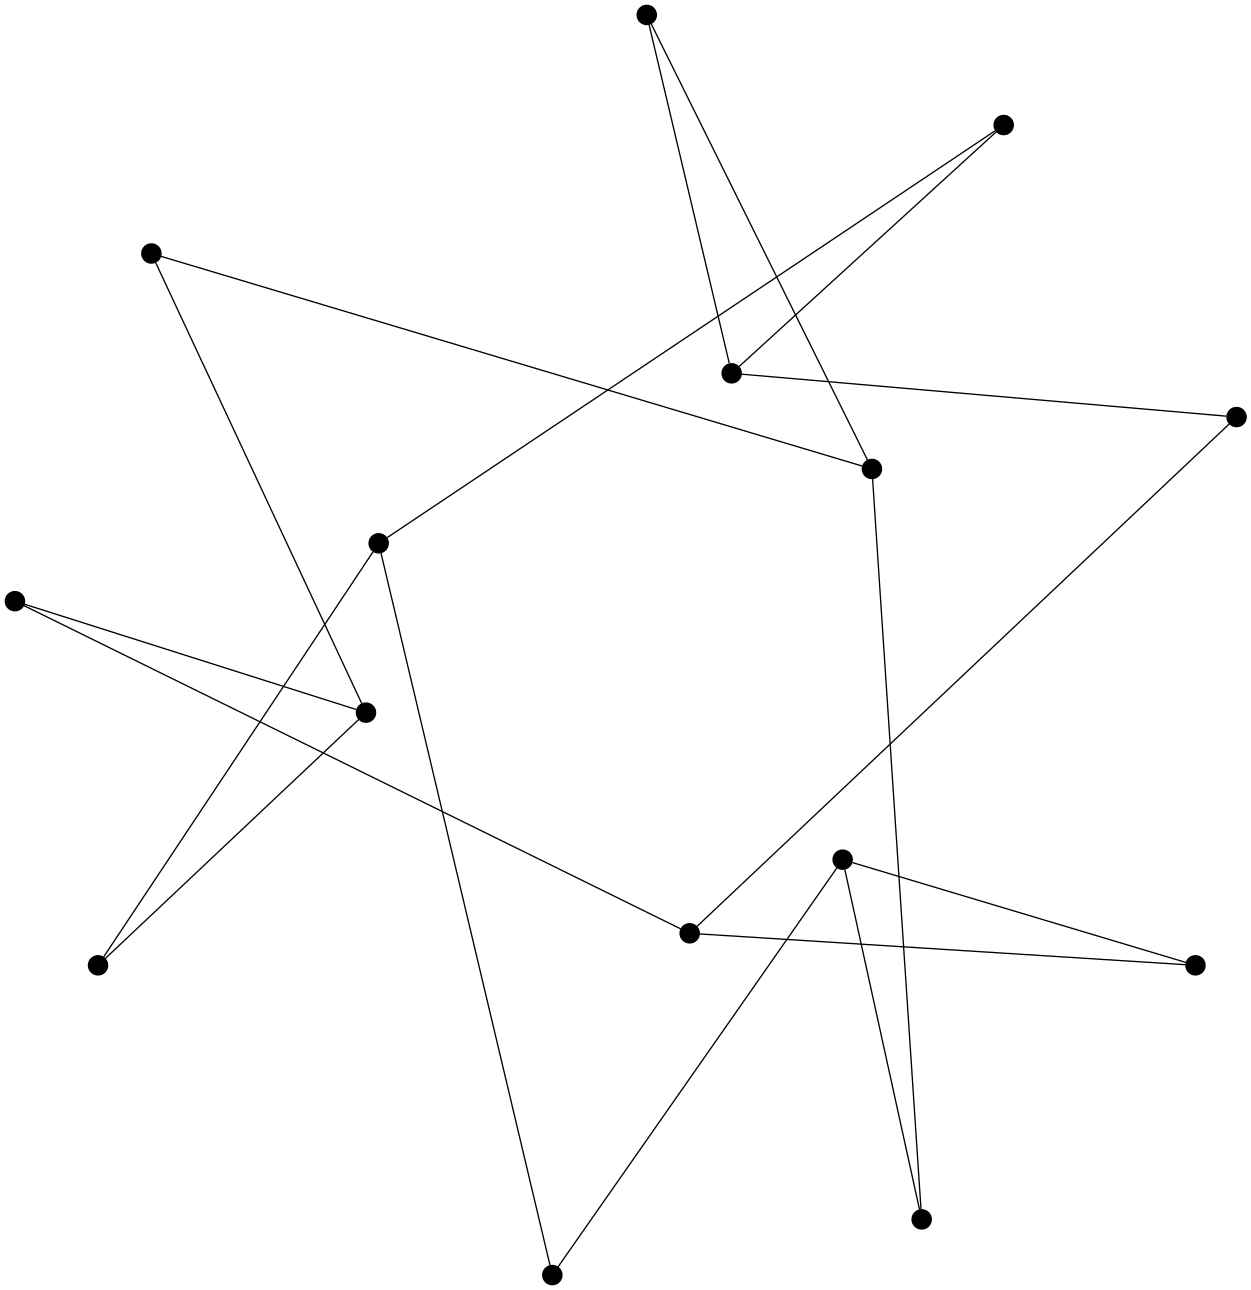
\includegraphics[scale=0.2]{graph_2.png}
    \caption{ (2,3)-regular bipartite graph with girth of 8. }
    \label{be_not_afraid}
\end{figure}

Bipartite graph with girth $14$ is shown in figure \ref{be_not_afraid_2}. It has 42 control and 63 informational vertices.

\begin{figure}[!h]
    \centering
    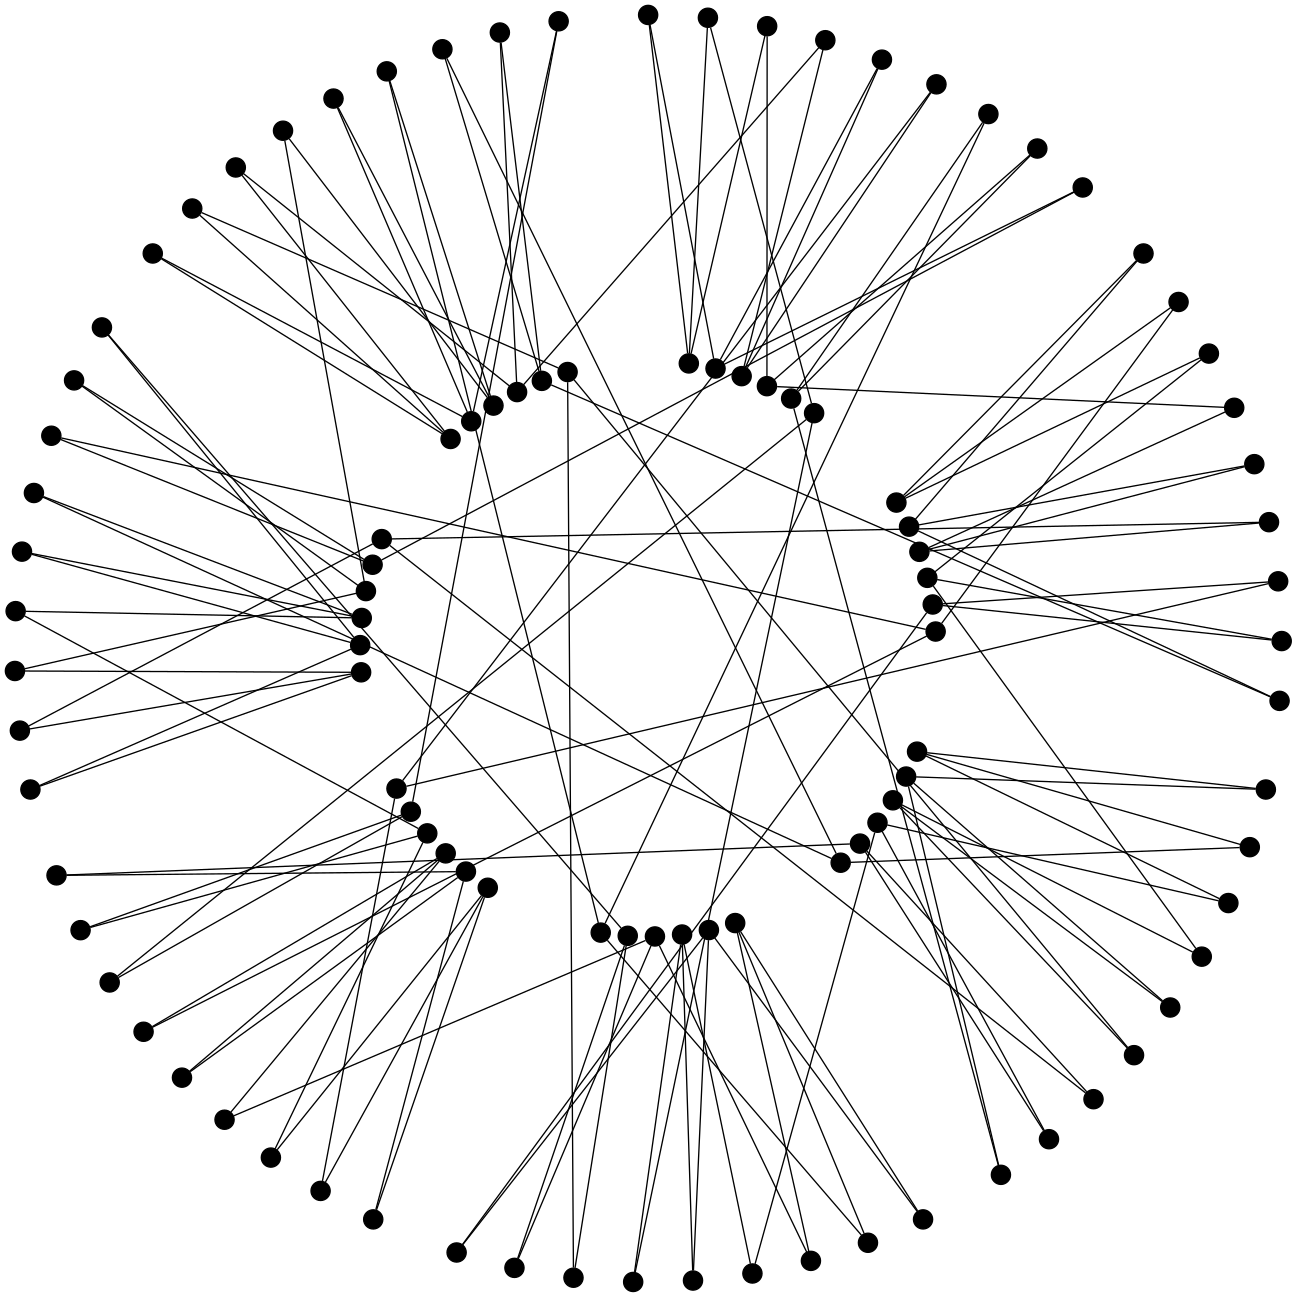
\includegraphics[scale=0.2]{graph_3.png}
    \caption{ (2,3)-regular bipartite graph with girth of 14. }
    \label{be_not_afraid_2}
\end{figure}

\section{Conclusion.}

% Посмотреть какие времена используются в заключениях в других статьях
% Проверить, подходит ли слово precise в этом контексте

In this article we have proposed a structural method for construction of bipartite graphs with any given girth by expanding metagraphs. The algorithm for selection of optimal weights for metagraphs was developed. Precise estimation of girth among all expansions of metagraph was given. Algorithm for iterative selection of metragraph structure was proposed.

These algorithms and theorems might in future be generalized for any graphs. Generalized algorithms can be used for construction of structured graphs with specific properties.

\begin{table}[H]
\caption{This is a table caption. Tabels should be placed in the main text
near to the first time they are cited. Table caption should be above
the the table.}

\centering{}%
\begin{tabular}{|c|c|c|}
\hline 
type & A & B\tabularnewline
\hline 
\hline 
expression & $\frac{a}{b}$ & $a+b$\tabularnewline
\hline 
expression & $a\cdot b$ & $\int f\left(x\right){\rm d}x$\tabularnewline
\hline 
\end{tabular}
\end{table}


\begin{thebibliography}{1}

%TODO: Proper references

%Fill the list of references in the alphabetical order here.
% Adopt the style like:

% \bibitem{bib1}
% {\small {\sc J. A. Baker:} {\it Isometries in normed spaces.}
% Amer. Math. Monthly, {\bf 78} (1971), 655--658.}

% \bibitem{bib2}
%  {\small {\sc A. Marshall, I. Olkin: }{\it Inequalities$:$ Theory of
% Majorization and Its Applications.} Academic Press, New York, 1979.}
% \end{thebibliography}

% \vspace{1cc}

% %Fill author(s) affiliation(s), address(es) and emails here:
% %example is shown
% \noindent
% {\bf John Doe}\\
% Department of Mathematics,\\
% University of Belgrade,\\
% Belgrade, Serbia\\
% E-mail: {\it joe.doe@mail.com}

% \vspace{0.1cc}

% \noindent
% {\bf Jane Doe}\\
% Department of Mathematics,\\
% University of Belgrade,\\
% Belgrade, Serbia\\
% E-mail: {\it jane.doe@mail.com}

% 1
\bibitem{zemor}
G. Zémor, On Expander Codes, IEEE Trans. on Information theory, IT-47
No 2, (2001) pp. 835–837.
  
% 2
\bibitem{johnson}
Johnson, Sarah. (2008). Introducing Low-Density Parity-Check Codes. 
% ~-- University of Newcastle, Australia, 2006.

% 3
\bibitem{gallager}
R. Gallager, "Low-density parity-check codes," in IRE Transactions on Information Theory, vol. 8, no. 1, pp. 21-28, January 1962, doi: 10.1109/TIT.1962.1057683

% 4
\bibitem{protographs}
J. Thorpe,
Low-density parity-check (LDPC) codes constructed from protographs.
~-- JPL, IPN Progress Rep., Aug. 2003, vol. 42–154.

% 5
\bibitem{skorohodov_reachability_problem}
Skorokhodov V.A. Generalization of the Reachability Problem on Directed Graphs
~-- Mathematics and Statistics, Vol. 8, No. 6, pp. 699 - 704, 2020. DOI: 10.13189/ms.2020.080610

% 6
\bibitem{tutte_graph_definition}
W.T. Tutte, Graph Theory. Cambridge University Press, Cambridge, 2001, 360 pp.
% https://books.google.rs/books?id=uTGhooU37h4C&printsec=frontcover#v=onepage&q&f=false

% 7
\bibitem{margulis_construction}
Margulis, G. A. (1982). Explicit constructions of graphs without short cycles and low density codes. Combinatorica, 2(1), 71–78. 
doi:10.1007/bf02579283
%% https://sci-hub.se/10.1007/bf02579283

% 9
%% Критика метода Маргулиса
\bibitem{margulis_critique}
David J.C. MacKay, Michael S. Postol, Weaknesses of Margulis and Ramanujan-Margulis Low-Density Parity-Check Codes, Electronic Notes in Theoretical Computer Science, Volume 74, 2003, Pages 97-104, ISSN 1571-0661, doi:10.1016/S1571-0661(04)80768-0.
% https://www.inference.org.uk/mackay/margulis.pdf

% 8
\bibitem{imrich_construction}
Imrich, W. (1984). Explicit construction of regular graphs without small cycles. Combinatorica, 4(1), 53–59. doi:10.1007/bf02579157 
%% https://sci-hub.se/10.1007/bf02579157

% 10
\bibitem{ldpc_encoding}
T. J. Richardson and R. L. Urbanke, "Efficient encoding of low-density parity-check codes," in IEEE Transactions on Information Theory, vol. 47, no. 2, pp. 638-656, Feb 2001, doi: 10.1109/18.910579

% 11
\bibitem{algebraic_aproach_to_sc_ldpc}
Beemer, A., Habib, S., Kelley, C. A., Kliewer, J. (2017). A generalized algebraic approach to optimizing SC-LDPC codes. In 55th Annual Allerton Conference on Communication, Control, and Computing, Allerton 2017 (pp. 672-679). (55th Annual Allerton Conference on Communication, Control, and Computing, Allerton 2017; Vol. 2018-January). Institute of Electrical and Electronics Engineers Inc. doi:10.1109/ALLERTON.2017.8262802

% https://web.njit.edu/~jkliewer/wp/paper/BHKK_Allerton17.pdf

% 12
\bibitem{lifts_of_graphs}
C. A. Kelley, "On codes designed via algebraic lifts of graphs," 2008 46th Annual Allerton Conference on Communication, Control, and Computing, Monticello, IL, USA, 2008, pp. 1254-1261, doi: 10.1109/ALLERTON.2008.4797704.

% https://typeset.io/pdf/on-codes-designed-via-algebraic-lifts-of-graphs-34h5sq5koc.pdf

% 13
\bibitem{vasic_combinatorial_construction}
B. Vasic and O. Milenkovic, "Combinatorial constructions of low-density parity-check codes for iterative decoding," in IEEE Transactions on Information Theory, vol. 50, no. 6, pp. 1156-1176, June 2004, doi: 10.1109/TIT.2004.828066.
% https://repository.arizona.edu/bitstream/handle/10150/641965/Combinatorial%20Constructions%20of%20Low-DensityParity-Check%20Codes%20for%20Iterative%20Decoding.pdf;jsessionid=9F016719B821C7D7CEBB9C48D7B37CB1?sequence=1

%14
\bibitem{Kim2002ExplicitCO}
Kim, Jon-Lark, Uri N. Peled, Irina G. Perepelitsa and Vera Pless. “Explicit Construction of Families of LDPC Codes with Girth at Least Six.” (2002).

\end{thebibliography}

\vspace{1cc}

\noindent
{\bf Oleg V. Arutyunov}\\
Institute of Mathematics, Mechanics and Computer Science,\\
Southern Federal University,\\
Rostov-on-Don, Russia\\
E-mail: {\it ArutunoffOleg@yandex.ru}

\vspace{0.1cc}

\noindent
{\bf Vladimir A. Skorokhodov}\\
Institute of Mathematics, Mechanics and Computer Science,\\
Southern Federal University,\\
Rostov-on-Don, Russia\\
E-mail: {\it vaskorohodov@sfedu,ru}


\end{document}
